
\subsection{Kompensation Störgröße Fahrzeug}

Bei einem stationären Fahrzeug genügt es, die Kopforientierung mittels \acs{IMU}-Daten der Brille zu bestimmen. Die gesuchte Kopforientierung relativ zum Fahrzeug stimmt dabei mit der Kopforientierung bezüglich der Weltkoordinaten überein. Sobald sich das Fahrzeug jedoch bewegt, wird die Schätzung der Kopforientierung verfälscht. Fährt das Fahrzeug beispielsweise eine Kurve, so wird die von der IMU gemessene Drehung als Änderung des Yaw-Winkels der Kopforientierung interpretiert, obwohl der Fahrer in Bezug zum Fahrzeug weiterhin geradeaus blickt.

Eine weitere Störquelle stellt die Fahrzeugelektronik und die damit einhergehenden Änderungen des Magnetfelds dar. Diese Störungen wirken sich negativ auf das zur Driftkorrektur eingesetzte Magnetometer aus (siehe Abschnitt XX \todo{richtigen Abschnitt referenzieren}).

Zur Korrektur der Fehlschätzung aufgrund der genannten Einflüsse wurden zwei Ansätze untersucht, die die Bestimmung der Kopforientierung relativ zum Fahrzeug stützen.

\begin{figure}[h]
  \centering
  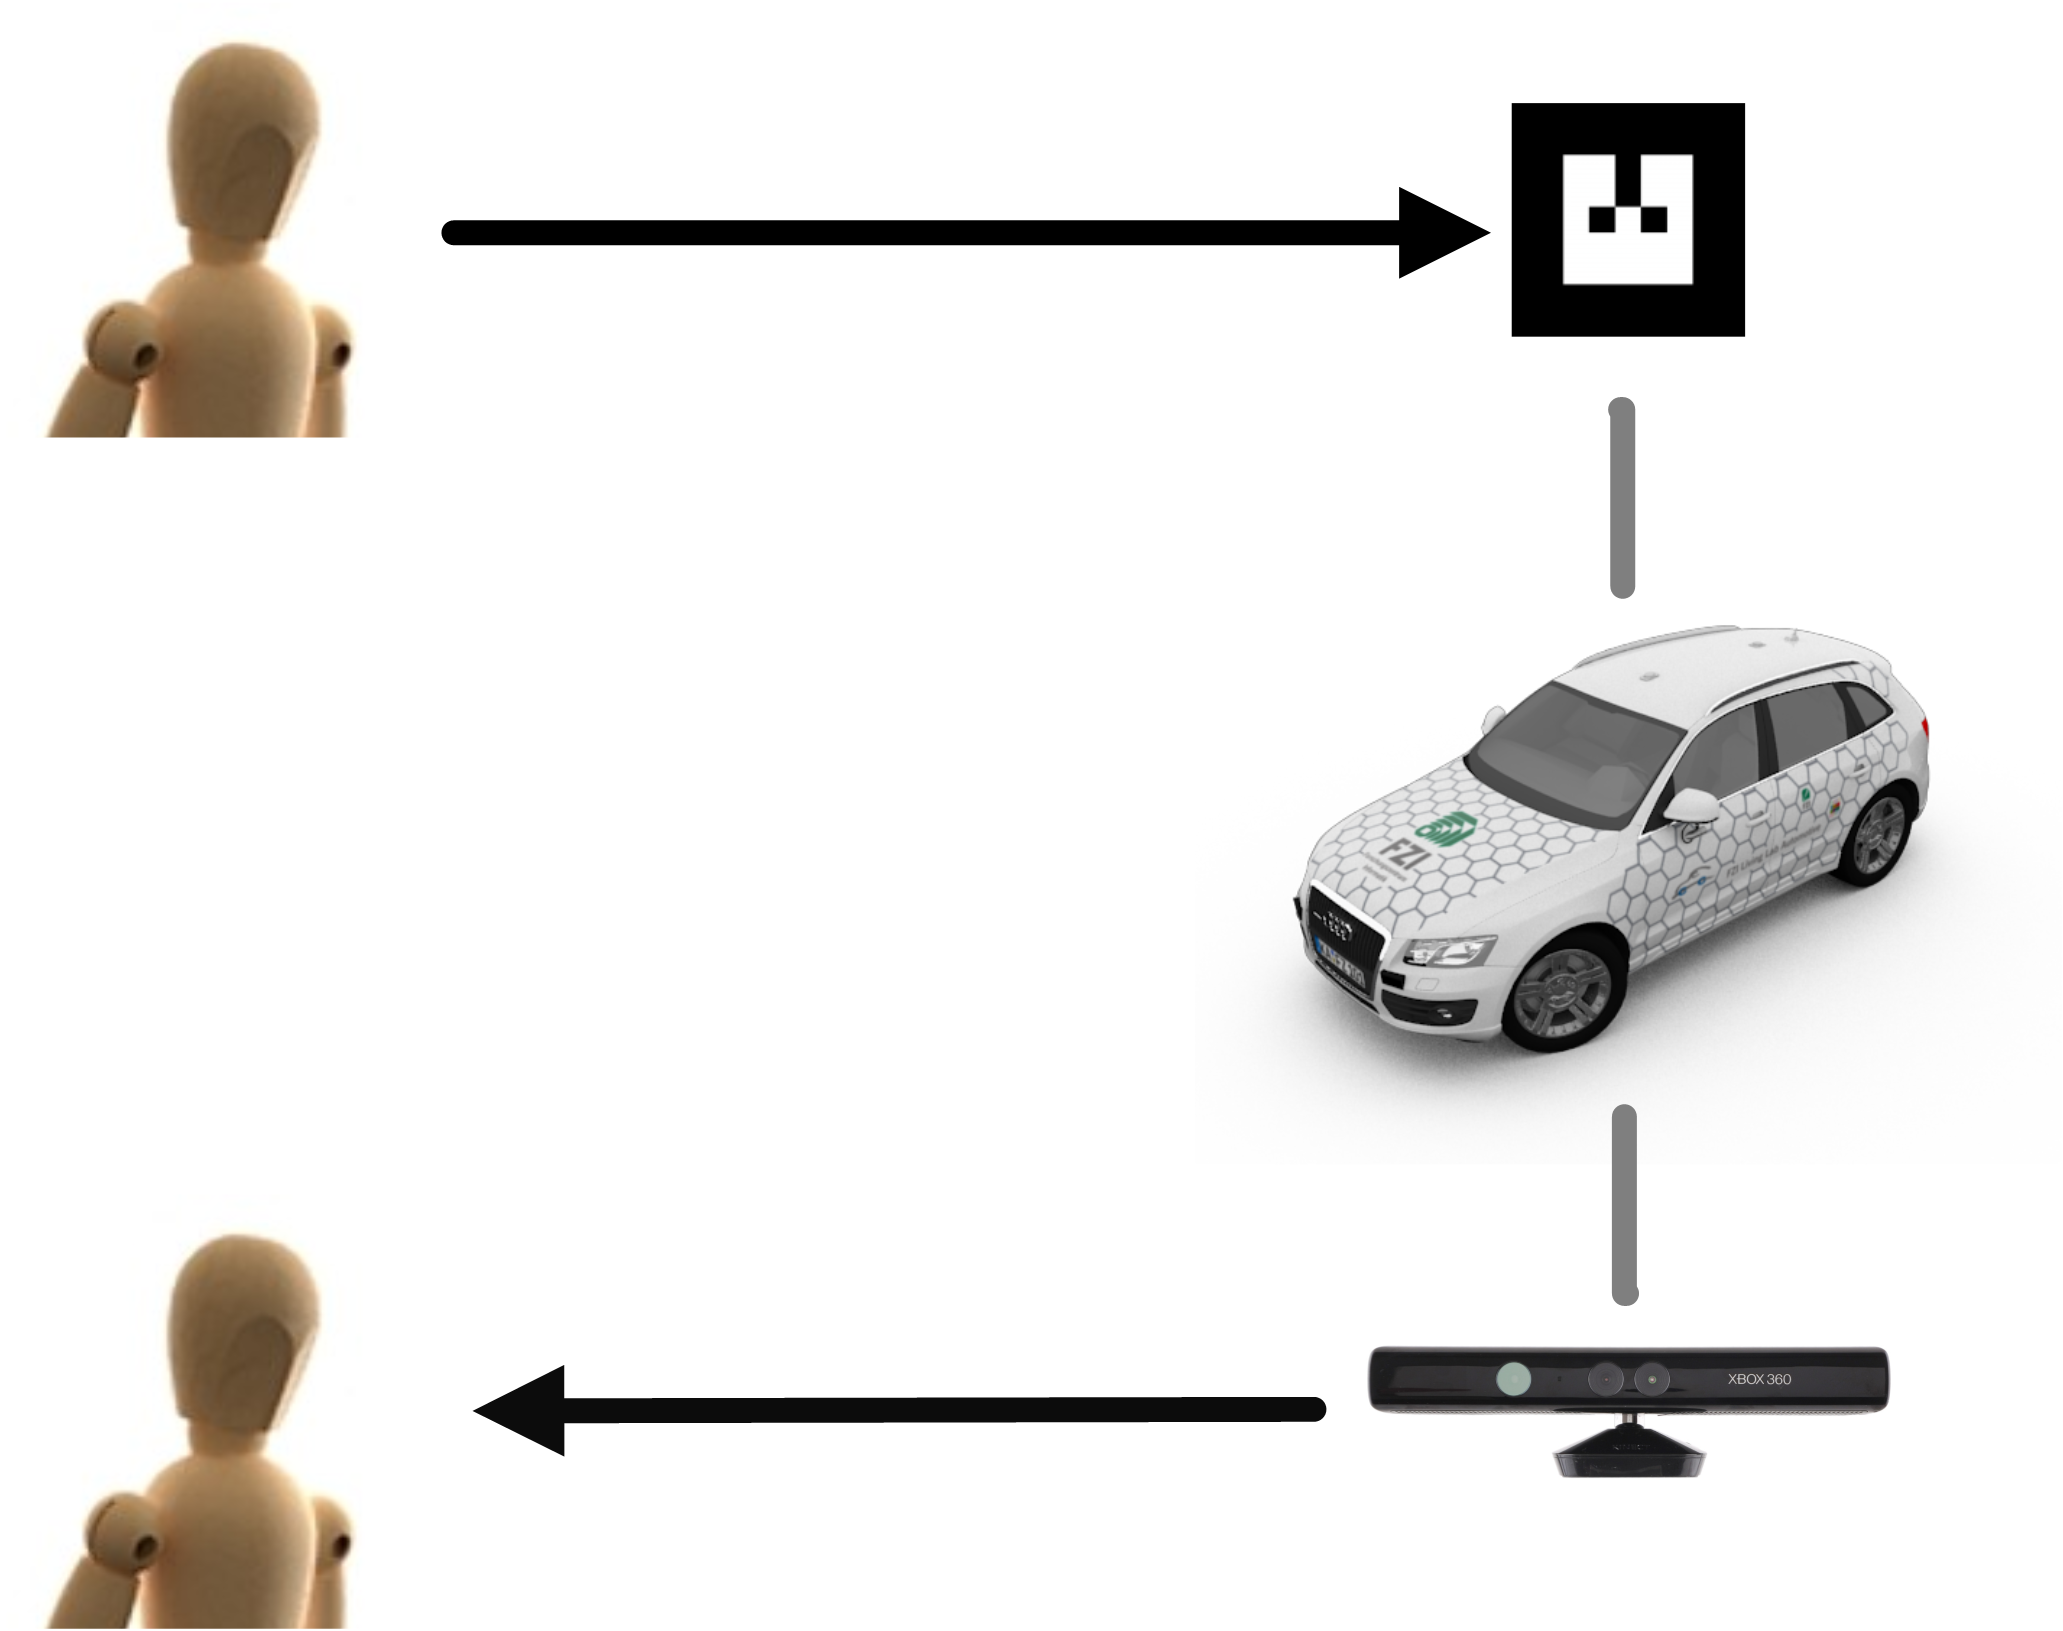
\includegraphics[width=0.4\textwidth]{Tracking_Ansaetze}
  \caption{Tracking-Ansätze: oben: stationärer Marker, bewegliche Kamera; unten: stationäre Kamera, bewegter Kopf}
  \label{fig:tracking_ansaetze}
\end{figure}

\subsubsection{Ansatz: Face-Tracking}



\subsubsection{Ansatz: Marker-Tracking}



\subsubsection{Fusion IMU und Marker-Tracking}
